\id{ГРНТИ 28.23.15}{}

\begin{articleheader}
\sectionwithauthors{М.Қ. Болсынбек, Г.Б. Абдикеримова, Ж.К. Тасжурекова, А.А.Адамов, С.К. Серикбаева, А.М. Ануарбеков}{ПРОГНОЗИРОВАНИЕ СОСТОЯНИЯ ПОЧВЫ В РАЗЛИЧНЫХ КЛИМАТИЧЕСКИХ ЗОНАХ
С ИСПОЛЬЗОВАНИЕМ МЕТОДОВ МАШИННОГО ОБУЧЕНИЯ}

{\bfseries
\textsuperscript{1}М.Қ. Болсынбек,
\textsuperscript{1}Г.Б. Абдикеримова,
\textsuperscript{2}Ж.К. Тасжурекова,
\textsuperscript{1}А.А.Адамов,
\textsuperscript{1}С.К. Серикбаева\textsuperscript{\envelope },
\textsuperscript{1}А.М. Ануарбеков
}
\end{articleheader}

\begin{affiliation}
\textsuperscript{1}Евразийский национальный университет имени Л.Н.Гумилева, Астана, Казахстан,

\textsuperscript{2}Таразский региональный университет им.М. Х. Дулати, Тараз, Казахстан

\raggedright \textsuperscript{\envelope }Корреспондент-автор: \href{mailto:inf_8585@mail.ru}{inf\_8585@mail.ru}
\end{affiliation}

В статье рассматривается применение методов машинного обучения для
прогнозирования состояния почвы в различных климатических зонах.
Прогнозирование состояния почвы является ключевым элементом управления
сельскохозяйственными и экологическими системами, поскольку состояние
почвы влияет на урожайность, биоразнообразие и способность поглощать
углерод. Традиционные методы мониторинга почвы требуют значительных
временных и ресурсных затрат, в то время как методы машинного обучения
позволяют обрабатывать большие объемы данных и строить модели,
учитывающие множество факторов, таких как климат, гидрология и
агротехнические практики. В статье представлены современные подходы к
использованию машинного обучения для анализа данных дистанционного
зондирования, таких как вегетационные индексы (NDVI, SAVI), альбедо и
индексы влажности почвы (MSI, NDMI). Эти методы помогают улучшить
точность прогнозов, выявить участки с высоким риском эрозии и предложить
меры для предотвращения деградации земель. Особое внимание уделено
возможности адаптации моделей к различным климатическим условиям, что
способствует устойчивому развитию сельского хозяйства и эффективному
управлению земельными ресурсами.

{\bfseries Ключевые слова:} прогнозирование состояния почвы, машинное
обучение, климатические зоны, дистанционное зондирование, эрозия,
вегетационные индексы, альбедо, влажность почвы.

\begin{articleheader}
{\bfseries МАШИНАЛЫҚ ОҚЫТУ ӘДІСТЕРІН ҚОЛДАНЫП ӘРТҮРЛІ КЛИМАТТЫҚ
АЙМАҚТАРДАҒЫ ТОПЫРАҚ ЖАҒДАЙЫН БОЛЖАУ}

{\bfseries
\textsuperscript{1}М.Қ. Болсынбек,
\textsuperscript{1}Г.Б. Абдикеримова,
\textsuperscript{2}Ж.К. Тасжурекова,
\textsuperscript{1}А.А.Адамов,
\textsuperscript{1}С.К. Серикбаева\textsuperscript{\envelope },
\textsuperscript{1}А.М. Ануарбеков
}
\end{articleheader}

\begin{affiliation}
\textsuperscript{1}Л.Н.Гумилев атындағы Еуразия ұлттық университеті, Астана, Қазақстан,

\textsuperscript{2}М.Х.Дулати атындағы Тараз өңірлік университеті, Тараз, Қазақстан,

e-mail: \href{mailto:inf_8585@mail.ru}{inf\_8585@mail.ru}
\end{affiliation}

Мақалада әртүрлі климаттық аймақтардағы топырақ жағдайын болжау үшін
машиналық оқыту әдістерін қолдану қарастырылады. Топырақ жағдайын болжау
ауылшаруашылық және экологиялық жүйелерді басқарудың негізгі элементі
болып табылады, өйткені топырақ жағдайы өнімділікке, биоәртүрлілікке
және көміртекті сіңіру қабілетіне әсер етеді. Топырақты бақылаудың
дәстүрлі әдістері айтарлықтай уақыт пен ресурстарды қажет етеді, ал
Машиналық оқыту әдістері үлкен көлемдегі деректерді өңдеуге және климат,
гидрология және агротехникалық тәжірибелер сияқты көптеген факторларды
ескеретін модельдер жасауға мүмкіндік береді. Мақалада вегетациялық
индекстер (NDVI, SAVI), альбедо және топырақ ылғалдылығы индекстері
(MSI, NDMI) сияқты қашықтықтан зондтау деректерін талдау үшін машиналық
оқытуды қолданудың заманауи тәсілдері келтірілген. Бұл әдістер
болжамдардың дәлдігін жақсартуға, эрозия қаупі жоғары жерлерді анықтауға
және жердің деградациясының алдын алу шараларын ұсынуға көмектеседі.
Ауыл шаруашылығының тұрақты дамуына және жер ресурстарын тиімді
басқаруға ықпал ететін модельдерді әртүрлі климаттық жағдайларға
бейімдеу мүмкіндігіне ерекше назар аударылады.

{\bfseries Түйін сөздер:} топырақ жағдайын болжау, машиналық оқыту,
климаттық аймақтар, қашықтықтан зондтау, эрозия, вегетациялық индекстер,
альбедо, топырақ ылғалдылығы.

\begin{articleheader}
{\bfseries FORECASTING SOIL CONDITIONS IN DIFFERENT CLIMATIC ZONES USING
MACHINE LEARNING METHODS}

{\bfseries
\textsuperscript{1}M.Bolsynbek,
\textsuperscript{1}G. Abdikerimova,
\textsuperscript{2}Zh. Taszhurekova,
\textsuperscript{1}A. Adamov,
\textsuperscript{1}S.Serikbayeva\textsuperscript{\envelope },
\textsuperscript{1}A. Anuarbekov
}
\end{articleheader}

\begin{affiliation}
\textsuperscript{1}L.N. Gumilyov Eurasian National University, Astana, Kazakhstan,

\textsuperscript{2}Taraz Regional University named after M.KH.Dulaty, Taraz, Kazakhstan,

e-mail: \href{mailto:inf_8585@mail.ru}{inf\_8585@mail.ru}
\end{affiliation}

The article discusses the application of machine learning methods for
predicting soil conditions in various climatic zones. Predicting soil
conditions is a key element of agricultural and ecological systems
management, as soil conditions affect yields, biodiversity and the
ability to absorb carbon. Traditional soil monitoring methods require
significant time and resource costs, while machine learning methods
allow you to process large amounts of data and build models that take
into account many factors such as climate, hydrology and agrotechnical
practices. The article presents modern approaches to using machine
learning to analyze remote sensing data, such as vegetation indices
(NDVI, SAVI), albedo and soil moisture indices (MSI, NDMI). These
methods help to improve the accuracy of forecasts, identify areas with a
high risk of erosion and propose measures to prevent land degradation.
Special attention is paid to the possibility of adapting models to
different climatic conditions, which contributes to the sustainable
development of agriculture and effective land management.

{\bfseries Keywords:} soil condition forecasting, machine learning,
climatic zones, remote sensing, erosion, vegetation indices, albedo,
soil moisture.

\begin{multicols}{2}
{\bfseries Введение.} Прогнозирование состояния почвы - это ключевой
элемент в управлении аграрными системами и экосистемами, поскольку оно
помогает оптимизировать производство сельскохозяйственной продукции,
поддерживать здоровье экосистем и минимизировать воздействие изменения
климата на землю.

Состояние почвы напрямую влияет на урожайность, биоразнообразие и
способность поглощать углерод, что делает её важным объектом
исследований в контексте устойчивого развития. Однако почвенные
характеристики сильно варьируются в зависимости от региона и
климатических условий, что усложняет задачу точного прогнозирования.
Различные климатические зоны представляют собой уникальные комбинации
температурных режимов, уровней осадков и влажности, что влияет на
структуру и состав почвы. Например, в тропических зонах почва часто
подвергается интенсивной эрозии и потерям питательных веществ из-за
обильных осадков, тогда как в аридных регионах возникает проблема
деградации и засоления почв вследствие недостатка влаги {[}1{]}. Эти
факторы делают крайне важным адаптацию методов прогнозирования к
конкретным климатическим условиям. Традиционные методы исследования
состояния почвы, такие как полевые исследования и лабораторный анализ,
занимают много времени и ресурсов, а также требуют значительного
человеческого участия. Эти методы обеспечивают детальные данные, но
имеют ограниченные возможности для масштабирования и прогнозирования в
режиме реального времени. В условиях изменяющегося климата и нарастающих
экологических проблем возникает потребность в новых подходах, которые
позволяют быстро и точно оценивать состояние почвы.

Машинное обучение и современные методы обработки данных предлагают
инновационные решения для анализа почвенных условий. С их помощью можно
обрабатывать большие объемы данных, извлекать полезные закономерности и
строить модели, способные учитывать многовариантные зависимости между
факторами, такими как климат, гидрология и агротехнические практики. Это
позволяет значительно улучшить точность и скорость прогнозирования
состояния почвы в различных условиях.

В последнее время появилось множество исследований, посвященных
применению машинного обучения для задач сельского хозяйства и экологии.
Эти исследования показывают, что алгоритмы машинного обучения могут
эффективно использовать исторические данные о климате, почвенных
характеристиках и урожайности для предсказания будущих изменений
состояния почвы {[}2{]}. Такой подход значительно улучшает управление
земельными ресурсами, минимизирует риск неурожаев и повышает
устойчивость сельского хозяйства к изменениям климата.

Важным преимуществом машинного обучения является возможность
использования разнородных источников данных. В задачи прогнозирования
состояния почвы могут быть включены данные дистанционного зондирования,
метеорологические измерения, результаты лабораторных анализов почвы и
данные полевых наблюдений. Комплексный подход к анализу этих данных
позволяет получить более точные и полные прогнозы. Один из наиболее
перспективных подходов в области машинного обучения для прогнозирования
состояния почвы - это использование глубоких нейронных сетей и моделей,
основанных на временных рядах. Такие модели могут учитывать временную
динамику изменения почвенных характеристик и их зависимости от
климатических факторов. Это особенно важно для регионов с резко
меняющимися условиями, где почва подвержена значительным колебаниям в
короткие промежутки времени {[}3{]}.

Применение методов машинного обучения для прогнозирования состояния
почвы может значительно повысить эффективность сельскохозяйственного
производства. Сельхозпроизводители могут получать более точные
рекомендации по внесению удобрений, орошению и другим агротехническим
мероприятиям. Это, в свою очередь, позволяет уменьшить затраты на
ресурсы и снизить негативное воздействие на окружающую среду, например,
за счет уменьшения использования химических удобрений и пестицидов.
Машинное обучение также играет важную роль в мониторинге деградации
почв. В условиях изменения климата, особенно в засушливых и
полузасушливых регионах, почва подвержена деградации, что приводит к
снижению её плодородности. Прогностические модели на основе машинного
обучения могут помочь выявить ранние признаки деградации и предложить
превентивные меры, направленные на сохранение и восстановление
почвенного покрова.

Оценка влажности почвы - один из ключевых показателей для оценки её
состояния. Методы машинного обучения могут использовать спутниковые
данные для прогнозирования уровня влажности на больших территориях. Это
позволяет обеспечить более точные данные для систем орошения, тем самым
улучшая управление водными ресурсами в сельском хозяйстве.

Кроме того, использование машинного обучения для прогнозирования
состояния почвы помогает бороться с опустыниванием. В регионах с
повышенной подверженностью засухам и эрозии почв машинное обучение может
стать мощным инструментом для предсказания критических моментов и
принятия необходимых мер по восстановлению почвенного покрова. Также
важным аспектом является возможность применения машинного обучения для
прогнозирования химического состава почвы. Наличие или отсутствие
определенных элементов в почве, таких как азот, фосфор и калий, напрямую
влияет на рост растений и урожайность. Прогностические модели могут
помочь определить, в каких регионах требуется дополнительное внесение
удобрений, а где почва достаточно насыщена питательными веществами.

Проблемы опреснения и засоления почвы также могут решаться с помощью
методов машинного обучения. Эти процессы часто наблюдаются в засушливых
регионах и приводят к значительному снижению плодородности почвы.
Прогностические модели могут помочь идентифицировать области с высоким
риском засоления и предложить подходящие агротехнические меры для борьбы
с этой проблемой {[}4{]}. В условиях изменения климата важную роль
играет возможность прогнозирования воздействия экстремальных погодных
условий на почву. С помощью машинного обучения можно предсказать, как
засухи, наводнения и другие аномальные климатические явления повлияют на
состояние почвы в конкретных регионах. Это поможет заблаговременно
разработать стратегии адаптации для сельскохозяйственного сектора.
Особое внимание стоит уделить проблеме эрозии почвы, которая является
одной из главных причин деградации земель. Машинное обучение может
помочь определить, какие регионы наиболее подвержены эрозии, и
предложить эффективные методы её предотвращения. Это особенно важно для
горных и прибрежных регионов, где почва наиболее уязвима к разрушению.

Использование методов машинного обучения для прогнозирования состояния
почвы также способствует более эффективному управлению
сельскохозяйственными ресурсами на уровне страны. Национальные и
региональные правительства могут использовать прогнозные модели для
разработки долгосрочных стратегий по управлению земельными ресурсами,
что будет способствовать устойчивому развитию сельского хозяйства.

Прогнозирование состояния почвы является важным аспектом сельского
хозяйства и экологии, поскольку позволяет оптимизировать использование
земельных ресурсов и обеспечивать устойчивое развитие аграрных регионов
{[}5{]}. В разных климатических зонах почва подвержена различным внешним
воздействиям, таким как колебания температуры, осадков и уровня
влажности, что существенно влияет на её физические и химические
свойства. С развитием технологий машинного обучения появилась
возможность автоматизировать процессы анализа данных о почве и климате,
что значительно ускоряет и улучшает прогнозы её состояния. Методы
машинного обучения позволяют обрабатывать большие объемы информации,
учитывать многочисленные факторы и выявлять скрытые закономерности, что
повышает точность и надежность прогнозов. В данной статье
рассматриваются современные подходы к использованию машинного обучения
для прогнозирования состояния почвы в различных климатических зонах.

{\bfseries Методы и материалы.} Модели машинного обучения, применяемые для
прогнозирования состояния почвы, включают в себя современные алгоритмы
анализа больших данных, такие как XGBoost и глубокие нейронные сети
(DNN). XGBoost (Extreme Gradient Boosting) представляет собой метод
градиентного бустинга, который использует ансамбль решающих деревьев для
повышения точности предсказаний. Основное преимущество XGBoost
заключается в его способности эффективно обрабатывать разнородные данные
и справляться с пропусками в выборках. В процессе обучения алгоритм
итеративно создает деревья решений, каждое из которых исправляет ошибки
предыдущего, минимизируя отклонения в прогнозах. Для обучения модели
используются параметры состояния почвы, полученные из данных
дистанционного зондирования, такие как индексы вегетации (NDVI, SAVI),
влажность (MSI, NDMI) и альбедо. Этот подход позволяет модели точно
определять стадии эрозии и прогнозировать риск деградации земель.

Для успешного обучения моделей машинного обучения, таких как XGBoost и
глубокие нейронные сети, необходима тщательная подготовка данных. Этот
процесс начинается с сбора данных из различных источников: спутниковых
снимков (Sentinel-2), метеорологических станций и полевых наблюдений.
Данные включают спектральные индексы (NDVI, SAVI, MSI, NDMI),
температуру, уровень осадков и характеристики почвы. Полученные данные
часто имеют разную структуру и формат, поэтому первым этапом является их
преобразование в единую форму. Это включает в себя стандартизацию единиц
измерения, синхронизацию временных меток и удаление дубликатов.

После этого выполняется обработка аномалий и пропусков данных. Временные
ряды спутниковых наблюдений иногда содержат пропущенные значения из-за
облачности или технических сбоев в получении снимков. Для заполнения
таких пробелов применяются методы интерполяции, либо используются более
сложные техники, например, временные нейронные сети, которые могут
предсказывать недостающие значения на основе предыдущих данных. Также на
этом этапе выявляются выбросы --- значения, сильно отклоняющиеся от
нормы, например, резкие скачки индекса NDVI в засушливых регионах. Эти
аномалии могут быть вызваны ошибками измерений или временными природными
явлениями. Для их устранения применяется метод IQR (Interquartile Range)
или Z-score, которые помогают отфильтровать атипичные значения.

Завершающим этапом подготовки данных является нормализация и
масштабирование признаков. Поскольку разные параметры (например,
температура, альбедо и индексы вегетации) имеют различные диапазоны
значений, это может влиять на процесс обучения моделей. Для приведения
всех признаков к единому масштабу применяются методы Min-Max Scaling
(масштабирование значений в диапазон {[}0, 1{]}) или Standard Scaling
(преобразование к стандартному нормальному распределению). Это
необходимо, чтобы алгоритмы, такие как XGBoost и нейронные сети, могли
правильно учитывать влияние каждого признака на предсказание, не отдавая
приоритеты параметрам с большими числовыми значениями. После
нормализации данные становятся готовыми для обучения моделей, что
повышает их точность и стабильность при прогнозировании эрозии почвы и
деградации земель.

Помимо XGBoost, для анализа временных изменений почвенных характеристик
применяются глубокие нейронные сети. В частности, архитектуры на основе
LSTM (Long Short-Term Memory) и GRU (Gated Recurrent Unit) позволяют
моделям учитывать временную зависимость данных. Это особенно важно для
мониторинга почвы в условиях меняющегося климата, когда влажность и
состояние растительного покрова могут резко изменяться. Модели LSTM и
GRU способны запоминать долгосрочные зависимости и предсказывать будущие
изменения почвы, основываясь на исторических данных. В качестве входных
данных используются временные ряды спектральных индексов, температуры,
уровня осадков и показателей влажности. Обучение моделей происходит на
больших наборах данных, что позволяет повысить точность прогнозов даже в
условиях изменчивого климата.

Для верификации и оценки точности моделей применяются метрики, такие как
Accuracy, Precision, Recall и F1-Score. Эти показатели помогают
определить, насколько точно модели идентифицируют стадии эрозии и
предсказывают ухудшение состояния почвы. Для повышения надежности
результатов используется метод кросс-валидации, при котором данные
разбиваются на несколько частей, и обучение модели происходит на
различных подвыборках. Такой подход позволяет избежать переобучения и
повысить обобщающую способность моделей на новых данных. Кроме того,
результаты прогнозирования визуализируются в виде картографических
моделей, где состояние почвы отображается по уровням эрозии, что
позволяет легко идентифицировать критические зоны для последующих
восстановительных мероприятий.

Для анализа эрозии почв используются различные методики дистанционного
зондирования, основанные на спектральных характеристиках почвы и
растительности. Один из наиболее эффективных методов - это использование
вегетационных индексов. Индексы, такие как NDVI (Normalized Difference
Vegetation Index) и SAVI (Soil Adjusted Vegetation Index), позволяют
оценить состояние растительности, что является ключевым фактором для
анализа эрозии. NDVI вычисляется на основе разности отражения ближнего
инфракрасного (NIR) и красного (Red) спектров, и его значения
варьируются от -1 до 1. Низкие значения NDVI могут указывать на
отсутствие растительности, что часто связано с эрозией почвы. SAVI - это
модификация NDVI, которая учитывает влияние почвы на отражательную
способность и лучше подходит для регионов с разреженной растительностью,
где почва доминирует в спектре.

Кроме того, важную роль в анализе эрозии играет вычисление альбедо ---
отношения отражённой солнечной радиации к падающей. Альбедо,
представляющее собой долю отраженного солнечного излучения от
поверхности, играет важную роль в анализе эрозии почвы. Этот параметр
влияет на температурные режимы почвы и, соответственно, на процессы
испарения и влагонакопления. В условиях низкого альбедо, поверхность
почвы поглощает больше солнечного тепла, что может способствовать её
пересыханию, уменьшению связности грунта и, как следствие, усилению
эрозионных процессов. Для эрозии почвы, особенно в засушливых или
полузасушливых регионах, где почва более подвержена разрушению, важно
учитывать влияние альбедо на физические процессы, такие как испарение и
высыхание поверхностных слоев. Повышение температуры поверхности почвы
может усилить её подверженность ветровой эрозии, особенно если почвенный
покров нарушен или недостаточно увлажнен {[}6{]}.

С другой стороны, высокое альбедо может снижать испарение и уменьшать
скорость высыхания почвы, что способствует сохранению влаги в верхних
слоях почвы. Однако избыточное отражение солнечной энергии также может
приводить к охлаждению почвы, что иногда отрицательно сказывается на
биологических процессах, таких как рост растительности, которая играет
важную роль в укреплении почвенного покрова и противодействии эрозии.

Вычисление альбедо при прогнозировании эрозии почвы с использованием
методов машинного обучения позволяет учитывать динамику изменения
температуры поверхности и её взаимодействие с другими факторами, такими
как влажность и ветер. Это дает возможность строить более точные модели
предсказания эрозионных процессов, что в свою очередь помогает
заблаговременно разрабатывать меры по защите и сохранению почв в
уязвимых регионах.

Альбедо может быть вычислено на основе мультиспектральных данных с
использованием комбинации различных спектральных каналов, таких как
синий (B2), красный (B4), ближний инфракрасный (B8) и коротковолновой
инфракрасный (SWIR, B11 и B12). Высокие значения альбедо могут указывать
на деградированные или эродированные земли, что особенно актуально для
регионов, подверженных ветровой эрозии.
\end{multicols}

%% ??????
(1)

\begin{multicols}{2}
Другим важным аспектом анализа эрозии является оценка влажности почвы,
поскольку она играет ключевую роль в стабильности почвенного покрова и
его подверженности эрозионным процессам. Влажность почвы влияет на её
структуру, плотность и способность противостоять воздействию внешних
факторов, таких как ветер и вода. Влажная почва обычно обладает большей
связностью и устойчивостью к эрозии, в то время как сухая почва
становится более рыхлой, что делает её уязвимой для разрушения.

Низкая влажность почвы способствует увеличению риска ветровой эрозии.
Когда почва пересыхает, её частицы становятся менее сцепленными и легче
поднимаются ветром, особенно на открытых или незащищенных участках.
Ветровая эрозия часто наблюдается в засушливых регионах и может привести
к значительным потерям верхнего плодородного слоя почвы, что оказывает
негативное влияние на сельское хозяйство и экосистемы.

С другой стороны, чрезмерное увлажнение почвы, особенно во время
проливных дождей или наводнений, может способствовать водной эрозии.
Вода смывает поверхностные слои почвы, унося с собой питательные
вещества и органические вещества, что приводит к деградации земель. В
условиях склона или неравномерного рельефа этот процесс может
ускоряться, вызывая образование оврагов и оползней {[}7{]}.

В рамках использования методов машинного обучения для анализа эрозии
почвы оценка влажности является важным параметром, который помогает
предсказывать эрозионные риски {[}8{]}. С помощью моделей машинного
обучения можно анализировать данные о влажности почвы, поступающие из
различных источников, таких как датчики влажности, спутниковые снимки и
метеорологические данные {[}9{]}. Это позволяет учитывать, как
пространственную, так и временную динамику изменений влажности почвы,
что помогает прогнозировать периоды повышенной уязвимости почв к
эрозионным процессам.

Другим важным аспектом анализа эрозии является оценка влажности
почвы. Методы, основанные на индексах влажности, таких как MSI
(Moisture Stress Index) и NDMI (Normalized Difference Moisture Index),
позволяют оценить влагозапас почвы и растительности. MSI рассчитывается
как отношение коротковолнового инфракрасного спектра (SWIR) к ближнему
инфракрасному спектру (NIR) и показывает степень стресса от нехватки
влаги. NDMI позволяет оценить содержание влаги в растительности и почве
на основе разности NIR и SWIR спектров. Оба этих индекса играют ключевую
роль в анализе состояния почвы, так как эродированные земли часто теряют
свою способность удерживать влагу, что приводит к их высыханию и
деградации. В совокупности с вычислением альбедо и вегетационными
индексами, анализ влажности почвы предоставляет полное представление о
состоянии почвы и её подверженности эрозионным процессам {[}10{]}.

Важность влажности почвы для выявления эрозии:

Влажность почвы является важным показателем для определения состояния
земли. С помощью дистанционного зондирования можно оценить влажность
почвы и отличить сухие эродированные земли от здоровых участков.

Индексы влажности почвы:

{\bfseries MSI (Moisture Stress Index)}: Этот индекс измеряет степень
влажности почвы. Низкие значения MSI указывают на влажную почву, а
высокие значения --- на сухую, что может указывать на эрозию.

\(MSI = \frac{SWIR}{NIR}\) (2)

Где:

SWIR (B11 в Sentinel-2) --- коротковолновой инфракрасный диапазон;

NIR (B8 в Sentinel-2) --- ближний инфракрасный диапазон.

{\bfseries NDMI (Normalized Difference Moisture Index)}: Этот индекс
оценивает влажность растительности и почвы. Низкие значения NDMI могут
указывать на сухие участки.

\(NDMI = \frac{NIR - SWIR}{NIR + SWIR}\) (3)

Где:

SWIR --- коротковолновой инфракрасный диапазон (B11);

NIR --- ближний инфракрасный диапазон (B8).

Комбинированная математическая формула с учетом альбедо, \emph{MSI}, и
\emph{NDMI}:

Пусть:

\emph{A} --- альбедо (обозначающее отражательную способность
поверхности);

\emph{MSI} --- индекс стресса по влажности (Moisture Stress Index);

\emph{NDMI} --- индекс влажности почвы (Normalized Difference Moisture
Index);

\emph{A\textsubscript{min }}и A\textsubscript{max} --- пороговые
значения альбедо для эрозированных земель;

\emph{MSI\textsubscript{min }}и \emph{MSI\textsubscript{max}} ---
диапазон значений индекса стресса по влажности (чем больше \emph{MSI},
тем суше почва);

\emph{NDMI\textsubscript{min }}и \emph{NDMI\textsubscript{max}} ---
диапазон значений NDMI (чем меньше NDMINDMINDMI, тем суше почва).
\end{multicols}

(4)

\begin{multicols}{2}
где:

---
нормализованное значение альбедо, которое указывает на степень
оголённости поверхности (чем ближе значение к A\textsubscript{max}, тем
выше вероятность эрозии);

---
нормализованное значение \emph{MSI}, которое указывает на степень
сухости почвы (чем выше MSIMSIMSI, тем суше почва);

---
нормализованное обратное значение NDMI, которое используется для учета
влажности почвы (чем ниже NDMI, тем суше почва).

(4) формаула учитывает {\bfseries альбедо} (высокое альбедо указывает на
оголённые, возможно эрозированные земли), {\bfseries сухость почвы по MSI}
(чем выше значение MSI, тем суше почва), и {\bfseries влажность почвы по
NDMI} (чем меньше NDMI, тем суше почва).

Итоговая комбинация этих факторов позволяет оценить вероятность наличия
эрозии: чем выше результат по формуле, тем больше вероятность того, что
участок земли эродирован.

{\bfseries Результаты и обсуждение.} На основе сегментации, выполненной с
использованием спектральных индексов, альбедо и оценки влажности почвы,
был сформирован набор данных для обучения модели машинного обучения.
Этот набор содержит детализированную информацию о состоянии земельных
участков, разделённых на четыре категории: «Норма», «Первая стадия
эрозии», «Вторая стадия эрозии» и «Третья стадия эрозии». Для
сегментации использовались индексы вегетации, такие как NDVI, альбедо
для оценки отражательной способности поверхности, а также индексы
влажности почвы MSI и NDMI. Эти параметры являются ключевыми для
определения состояния земель и прогнозирования процессов эрозии.

Набор данных был построен на основе временных наблюдений, включающих
значения вегетационных индексов, альбедо и влажности почвы для каждого
участка. В каждом наблюдении фиксировались дата съемки, индекс NDVI,
отражающий уровень вегетации, альбедо - показатель отражения солнечного
излучения, MSI - индикатор стрессового состояния почвы по влажности, и
NDMI, оценивающий содержание влаги. Эти показатели обеспечивают
структуру данных для эффективного обучения моделей машинного обучения.

Каждая строка данных включает информацию о состоянии почвы и её
классификации в одну из четырёх категорий:


1. Норма: Участки с плотным растительным покровом, умеренным
альбедо и стабильной влажностью почвы. NDVI обычно варьируется от 0.3
до 0.6, что указывает на хорошую вегетацию. Альбедо низкое из-за
высокой абсорбции солнечной радиации. MSI и NDMI находятся в пределах
нормы, что говорит о достаточной влажности почвы.

1. Первая стадия эрозии: Земли с начальной деградацией.
Растительный покров истончается, NDVI находится в диапазоне 0.2--0.3.
Альбедо повышено, поскольку оголённая почва начинает отражать больше
солнечной энергии. MSI свидетельствует о дефиците влаги, что
способствует эрозионным процессам.

1. Вторая стадия эрозии: Значительное снижение вегетации. NDVI
снижается до 0.1--0.2, альбедо увеличивается, отражая потерю
растительности. MSI указывает на высокую сухость почвы, что затрудняет
её восстановление.

1. Третья стадия эрозии: Полная деградация земель. NDVI ниже
0.1, что свидетельствует о почти полном отсутствии растительности.
Альбедо превышает 0.3, а MSI и NDMI указывают на сильную сухость и
дефицит влаги. Эти земли требуют немедленного восстановления.
Набор данных был построен на основе спутниковых снимков с использованием
комбинации индексов NDVI, MSI, NDMI и альбедо, что позволило
классифицировать земельные участки по стадиям эрозии. Данные содержат
параметры, такие как дата наблюдения, значения NDVI, альбедо, MSI, NDMI
и класс эрозии. Это помогает прогнозировать дальнейшее развитие
эрозионных процессов и разрабатывать меры по восстановлению
деградированных земель.

Набор данных был создан на основе сегментации изображений, выполненной с
применением комбинации вегетационных индексов, таких как NDVI, SI, NDMI,
MSI, и значений альбедо. Это позволило классифицировать почвы по уровням
эрозии, разделив их на разные категории. Сегментация опиралась на
научные методы анализа растительности и почвы, что дало возможность
точно оценить степень деградации земель. В результате выделены четыре
класса, отражающие различные стадии эрозии.


1. Первый класс - "Норма". Этот класс включает земли, где эрозия
отсутствует или проявляется минимально. Земли находятся в
удовлетворительном состоянии, и на них наблюдаются нормальные процессы
вегетации. В данной категории содержится 1,775,535 экземпляров.

1. Второй класс - "Начальная стадия эрозии". В эту категорию входят
земли, на которых начинают проявляться первые признаки эрозии, такие
как потеря растительности или начальная деградация почвы. В этой
категории насчитывается 4,989 экземпляров.

1. Третий класс - "Средняя стадия эрозии". Данная категория включает
земли, на которых наблюдаются более выраженные признаки эрозии. Почвы
теряют способность удерживать влагу, а значения альбедо и MSI
повышаются. Эти земли требуют серьёзных мер по восстановлению. В этой
группе содержится 56,110 экземпляров.

1. Четвёртый класс - "Критическая стадия эрозии". Почвы в этой категории
почти полностью деградированы, они не способны удерживать влагу и
имеют высокие значения альбедо и MSI, что указывает на критическую
сухость и отсутствие растительности. Земли в этой категории
подвергаются сильным разрушительным процессам, таким как выветривание
и потеря плодородного слоя. В данной категории содержится 7,517
экземпляров.
Структура данных для каждого участка земли включает следующие параметры:

Дата получения спутникового снимка - важнейший параметр для анализа
временных изменений в динамике эрозии.

Индекс NDVI - показывает состояние растительности на участке: высокие
значения свидетельствуют о густой растительности, низкие -об её
отсутствии.

Индекс SI (Soil Index) - характеризует состояние почвы, вычисляется как
отношение красного канала к ближнему инфракрасному диапазону и позволяет
выявлять деградированные участки.

Альбедо - отражает способность поверхности отражать солнечное излучение:
высокие значения характерны для оголённых почв, низкие - для покрытых
растительностью.

Индекс MSI (Moisture Stress Index) - оценивает содержание влаги в почве;
высокие значения указывают на сильный водный стресс.

Индекс NDMI (Normalized Difference Moisture Index) - показывает уровень
влажности растительности и почвы, основанный на ближнем и среднем
инфракрасных диапазонах, и используется для оценки водного стресса.

Каждый участок классифицируется по уровню эрозии, обозначенному как
ErosionClass (0 - норма, 1 - начальная стадия эрозии, 2 - средняя стадия
эрозии, 3 - критическая стадия эрозии). Эта структура данных позволяет
проводить комплексный анализ земель, прогнозировать развитие эрозионных
процессов и разрабатывать меры по восстановлению деградированных
территорий.

После того как были применены различные методы анализа, все данные были
использованы для создания набора данных для машинного обучения.
Спектральные данные, включая вегетационные индексы, альбедо и индексы
влажности, были объединены для обучения моделей машинного обучения. Эти
данные включали множество различных спектральных характеристик, которые
указывали на наличие или отсутствие эрозии на различных участках земли.
Комбинированный анализ позволил выявить ключевые закономерности в
изменении почвы под воздействием эрозии и создать качественный набор
данных для обучения моделей.

На рисунке 1 представлено исходное изображение, полученное с
использованием спутника Sentinel-2. Оно демонстрирует регион, где
различимы участки с разными состояниями земель. На изображении можно
увидеть, как плодородные земли с плотным растительным покровом, так и
пустые участки, которые могут быть либо обработаны, либо находиться под
паром. Эти различия в типах земель позволяют использовать данные для
анализа состояния почвы и растительности, что является важным шагом для
сегментации и последующей классификации уровня эрозии.
\end{multicols}


\begin{figure}[H]
	\centering
	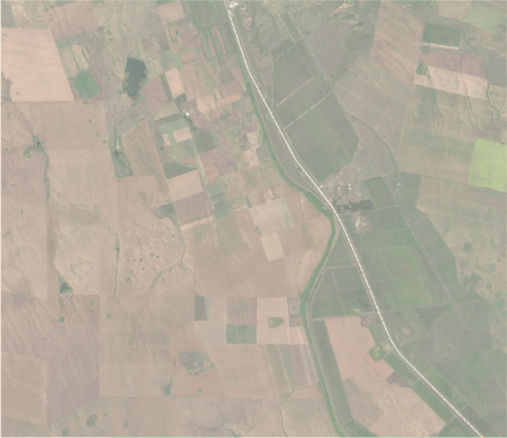
\includegraphics[width=0.8\textwidth]{media/ict/image31}
	\caption*{}
\end{figure}


\begin{figure}[H]
	\centering
	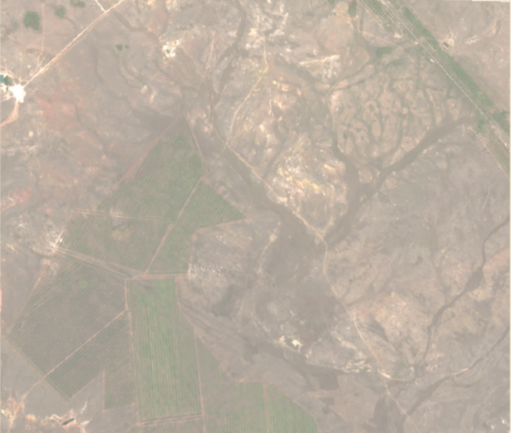
\includegraphics[width=0.8\textwidth]{media/ict/image32}
	\caption*{}
\end{figure}


{\bfseries Рис.1 - Оригинальное изображение}

\begin{multicols}{2}
Этот снимок является основой для дальнейшего анализа состояния почвы и
оценки эрозионных процессов с применением спектральных индексов. Он
предоставляет исходные данные, которые затем обрабатываются для
выявления признаков эрозии.

На рисунке 2 представлено изображение, которое демонстрирует результат
вычисления альбедо - метода, оценивающего способность поверхности
отражать солнечное излучение. На этом изображении участки земли с
разными уровнями альбедо выделены различными цветами, где более светлые
оттенки указывают на высокие значения альбедо. Такие участки, как
правило, соответствуют оголённым или эродированным землям, которые
теряют способность поглощать солнечную энергию и отражают её в большей
степени. Этот метод позволяет идентифицировать участки, подверженные
эрозионным процессам, и оценивать степень их деградации. На изображении
видно, что большая часть земель окрашена в жёлтый цвет, что указывает на
высокие значения альбедо. Это часто связано с эродированными или
оголёнными участками, где отсутствует растительный покров, что приводит
к повышенной отражательной способности поверхности. Такие участки
требуют особого внимания при прогнозировании эрозионных процессов.
\end{multicols}


\begin{figure}[H]
	\centering
	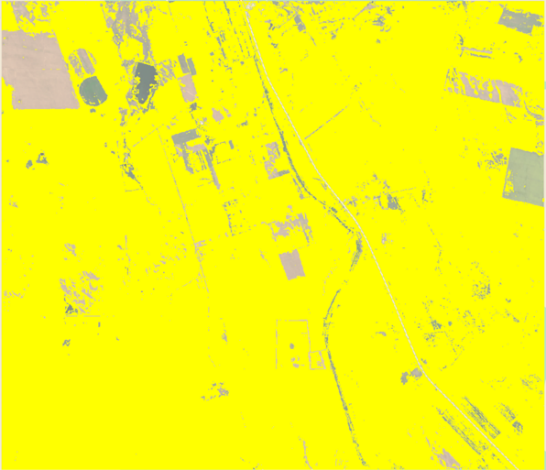
\includegraphics[width=0.8\textwidth]{media/ict/image33}
	\caption*{}
\end{figure}


\begin{figure}[H]
	\centering
	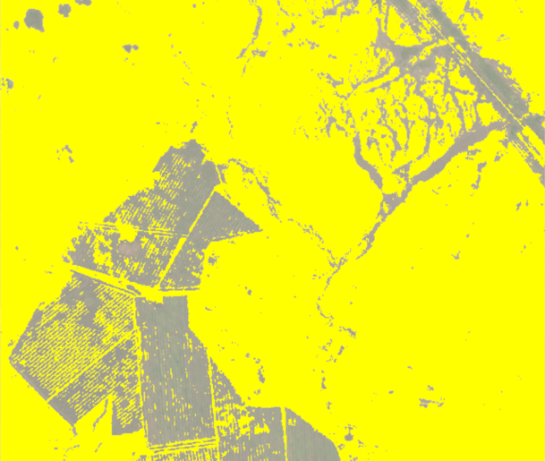
\includegraphics[width=0.8\textwidth]{media/ict/image34}
	\caption*{}
\end{figure}


{\bfseries Рис.2. - Использование метода альбедо}

\begin{multicols}{2}
Этот метод показывает, что почти вся поверхность земли обладает высоким
отражением, что может свидетельствовать о возможной эрозии. Однако это
не всегда верный признак. Некоторые участки, кажущиеся эродированными,
на самом деле могут быть паровыми землями, где уже был собран урожай.
Эти земли временно пусты, но могут сохранять достаточный уровень
влажности. Поэтому метод альбедо может приводить к ложноположительным
результатам, неверно интерпретируя плодородные или временно пустующие
земли как эродированные.

На рисунке 3 представлены три категории эрозии земель, отображённые с
использованием различных оттенков. Для анализа был применён
комбинированный метод, включающий несколько показателей: NDVI (индекс
вегетации), альбедо (отражательная способность), MSI (индекс стресса по
влажности) и NDMI (индекс влажности почвы). Эти индексы обеспечивают
комплексную оценку состояния земель и помогают распределить их по
категориям в зависимости от степени деградации.
\end{multicols}


\begin{figure}[H]
	\centering
	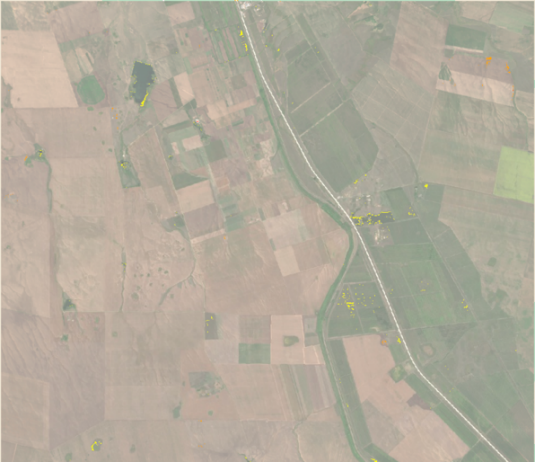
\includegraphics[width=0.8\textwidth]{media/ict/image35}
	\caption*{}
\end{figure}


\begin{figure}[H]
	\centering
	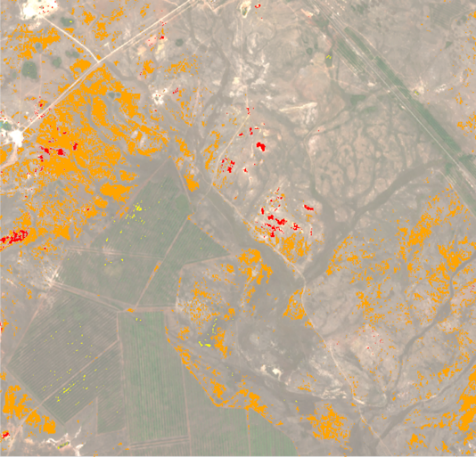
\includegraphics[width=0.8\textwidth]{media/ict/image36}
	\caption*{}
\end{figure}


{\bfseries Рис.3 - Использование комбинированного метода (альбедо + оценка влажности})

\begin{multicols}{2}
Жёлтая область на рисунке 3 указывает на участки, находящиеся на первой
степени эрозии (начальная стадия). В этих зонах наблюдается снижение
индекса NDVI, что свидетельствует о начале деградации растительного
покрова, и умеренные значения альбедо, указывающие на повышение
отражательной способности поверхности. Это начальные признаки того, что
почва становится более уязвимой к эрозии. Дополнительные параметры,
такие как MSI (индекс сухости) и NDMI (индекс влажности), также
показывают, что почва начинает пересыхать, что может способствовать
дальнейшему ухудшению её состояния. Если не принять меры для
восстановления земель на этой стадии, эрозионные процессы могут
усилиться. Условия для первой степени эрозии включают NDVI в диапазоне
от 0.2 до 0.5, что указывает на среднее состояние растительности,
альбедо от 0.1 до 0.2, характеризующее умеренную отражательную
способность, и MSI от 0.8 до 1.5, что свидетельствует о умеренной
сухости почвы.

Оранжевые участки на изображении указывают на среднюю степень эрозии
почвы, что означает начавшийся процесс её деградации. Почва на этих
участках теряет способность поддерживать здоровый растительный покров, и
NDVI, характеризующий плотность растительности, здесь ниже, чем на
начальной стадии эрозии. Одновременно с этим увеличивается альбедо, что
указывает на оголённые или мало защищённые почвенные поверхности, более
подверженные воздействию солнечного излучения. Высокие значения MSI
(индекс сухости) и низкие NDMI (индекс влажности) свидетельствуют о том,
что почва испытывает повышенный дефицит влаги, что ускоряет эрозионные
процессы. Условия для второй степени эрозии включают NDVI в диапазоне от
0.1 до 0.3, что указывает на низкий уровень растительности, альбедо от
0.2 до 0.25, характеризующее повышенную отражательную способность
поверхности, и MSI выше 1.5, что свидетельствует о высокой сухости
почвы. На этих участках уже можно наблюдать серьёзные признаки
деградации, и, если не принять своевременные меры, ситуация может
ухудшиться, вплоть до перехода к более тяжёлым стадиям эрозии.

Красные участки на изображении указывают на высокую степень эрозии, где
почва сильно деградировала и растительный покров практически
отсутствует. Высокие значения альбедо указывают на оголённую,
незащищённую почву, а высокие MSI и низкие NDMI свидетельствуют о полной
потере влаги. Такие земли считаются непригодными для
сельскохозяйственного использования без серьёзных восстановительных
мероприятий. Условия для третьей степени эрозии включают NDVI менее 0.1,
что означает очень низкий или отсутствующий растительный покров, альбедо
выше 0.25, что характеризует очень высокую отражательную способность, и
MSI выше 1.5, свидетельствующий о крайне высокой сухости почвы.

На следующем, 4 рисунке, представлена полная сегментация земель на
четыре категории в зависимости от их состояния. Зелёные области
указывают на земли в нормальном состоянии, где эрозия отсутствует, а
почва остаётся пригодной для сельскохозяйственного использования. Эти
участки демонстрируют нормальные показатели вегетации (NDVI), умеренное
альбедо и стабильную влажность почвы, что свидетельствует об устойчивом
и здоровом состоянии почвенного покрова.
\end{multicols}

\begin{figure}[H]
	\centering
	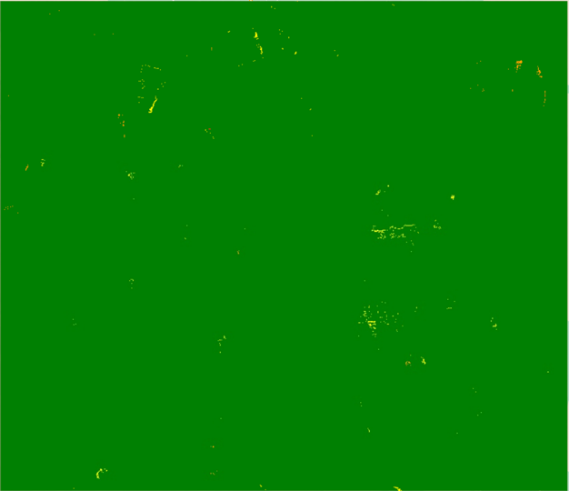
\includegraphics[width=0.8\textwidth]{media/ict/image37}
	\caption*{}
\end{figure}


\begin{figure}[H]
	\centering
	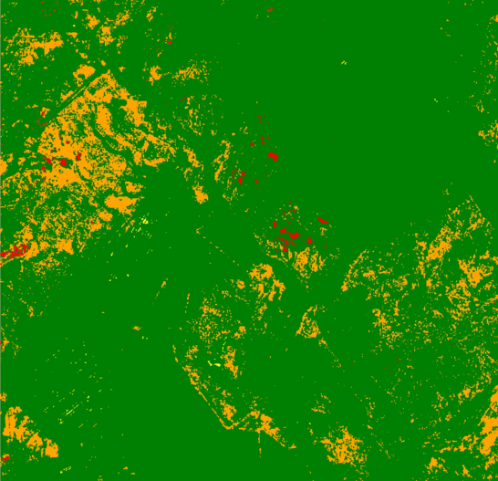
\includegraphics[width=0.8\textwidth]{media/ict/image38}
	\caption*{}
\end{figure}


{\bfseries Рис.4 - Полная сегментация, зелёные участки это норма, жёлтые
это начальная стадия, оранжевая это прогресс эрозии, красная это уже
деградированные земля то есть непригодная земля}

\begin{multicols}{2}
Жёлтые, оранжевые и красные участки на изображении представляют собой
земли, подверженные различным стадиям эрозии: жёлтые области указывают
на начальную стадию, где почва уже демонстрирует первые признаки сухости
и деградации растительного покрова, но всё ещё может быть восстановлена
при правильном управлении; оранжевые области отражают среднюю стадию
эрозии, при которой почва потеряла значительную часть своей
плодородности, что сопровождается увеличением альбедо, снижением
влажности и ослаблением растительности; красные области свидетельствуют
о высокой стадии эрозии, где почва почти полностью утратила свою
пригодность для сельскохозяйственного использования, а её восстановление
требует значительных усилий, о чём говорят высокое альбедо и низкие
показатели индексов влажности.

Важно отметить, что такие элементы, как дороги, искусственные
сооружения, дома и другие постройки на изображении не учитываются в
анализе. Они автоматически классифицируются как "норма" (зелёный цвет) и
исключаются из расчётов при оценке состояния почвы, поскольку не
являются частью сельскохозяйственных или природных земель. Алгоритм
сегментации распознаёт эти объекты как неподверженные эрозии и не
включает их в анализ деградации почв. Благодаря сегментации удалось
получить более чёткое и наглядное представление о состоянии земель,
позволяя увидеть, какие территории требуют внимания и проведения
восстановительных мероприятий для предотвращения дальнейшей эрозии и
деградации. Особенно важно, что нормальные участки почвы (зелёные)
выделяются как потенциальные зоны, которые можно сохранить и защитить от
будущего ухудшения состояния.

Применение технологий машинного обучения оказалось крайне эффективным
для анализа и прогнозирования процессов эрозии почвы. Одним из наиболее
успешных методов, использованных в исследовании, стал алгоритм XGBoost,
основанный на градиентном бустинге. Данный метод позволяет выявлять
сложные взаимосвязи между различными входными параметрами, такими как
спектральные индексы, альбедо и показатели влажности, и целевыми
переменными --- например, наличие эрозии. XGBoost был выбран за его
способность справляться с большими объемами данных и за высокую
точность, что важно при анализе многофакторных природных явлений.
Преимуществом XGBoost является устойчивость к переобучению, что
позволяет создавать модели, которые сохраняют высокую точность на
различных типах данных.

Для обучения модели использовались данные дистанционного зондирования,
включающие показатели вегетации, альбедо и влажности почвы. Обученная
модель продемонстрировала высокую способность к обобщению, так как
данные охватывали различные типы почв и климатические зоны, что
позволило модели точно прогнозировать эродированные участки. Было
установлено, что наибольшую точность прогнозирования эрозии, особенно в
зонах, подверженных ветровой эрозии, давали комбинированные методы
анализа альбедо и влажности. Таким образом, использование методов
машинного обучения в сочетании с данными спутникового мониторинга
открывает новые возможности для точного и оперативного мониторинга
состояния почвы и предотвращения её деградации.
\end{multicols}

\begin{figure}[H]
	\centering
	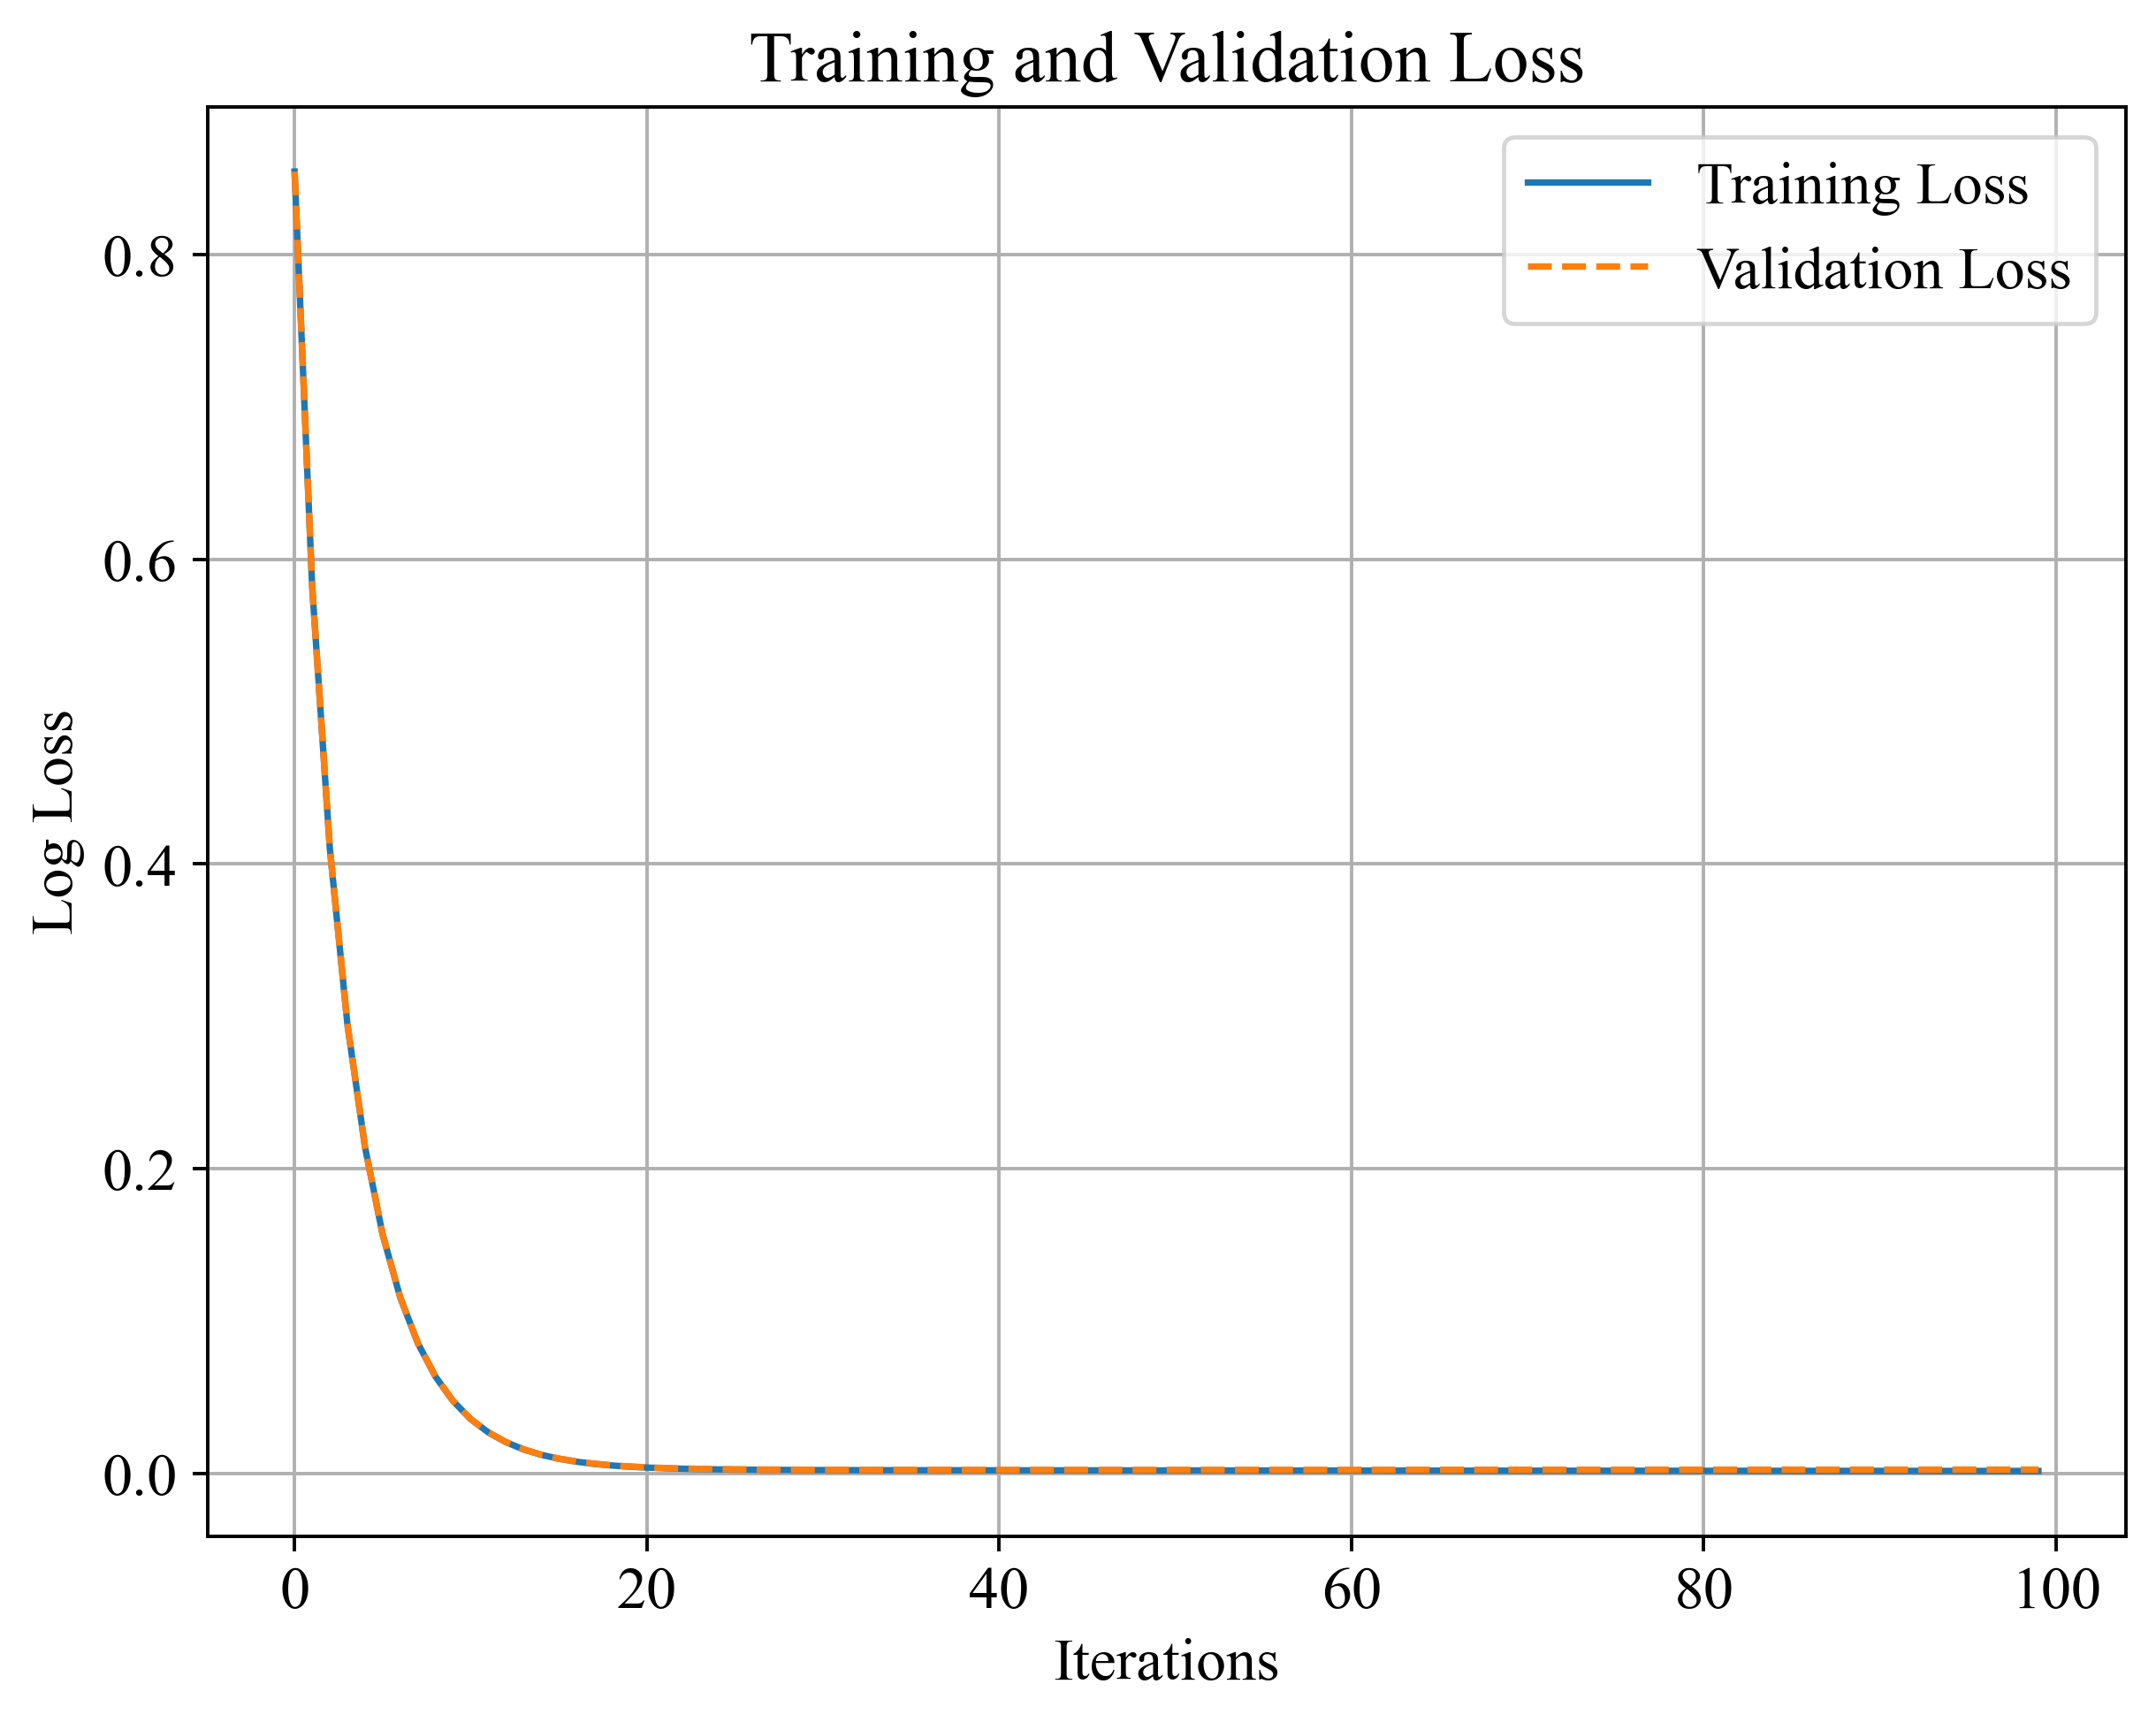
\includegraphics[width=0.8\textwidth]{media/ict/image39}
	\caption*{}
\end{figure}

\begin{figure}[H]
	\centering
	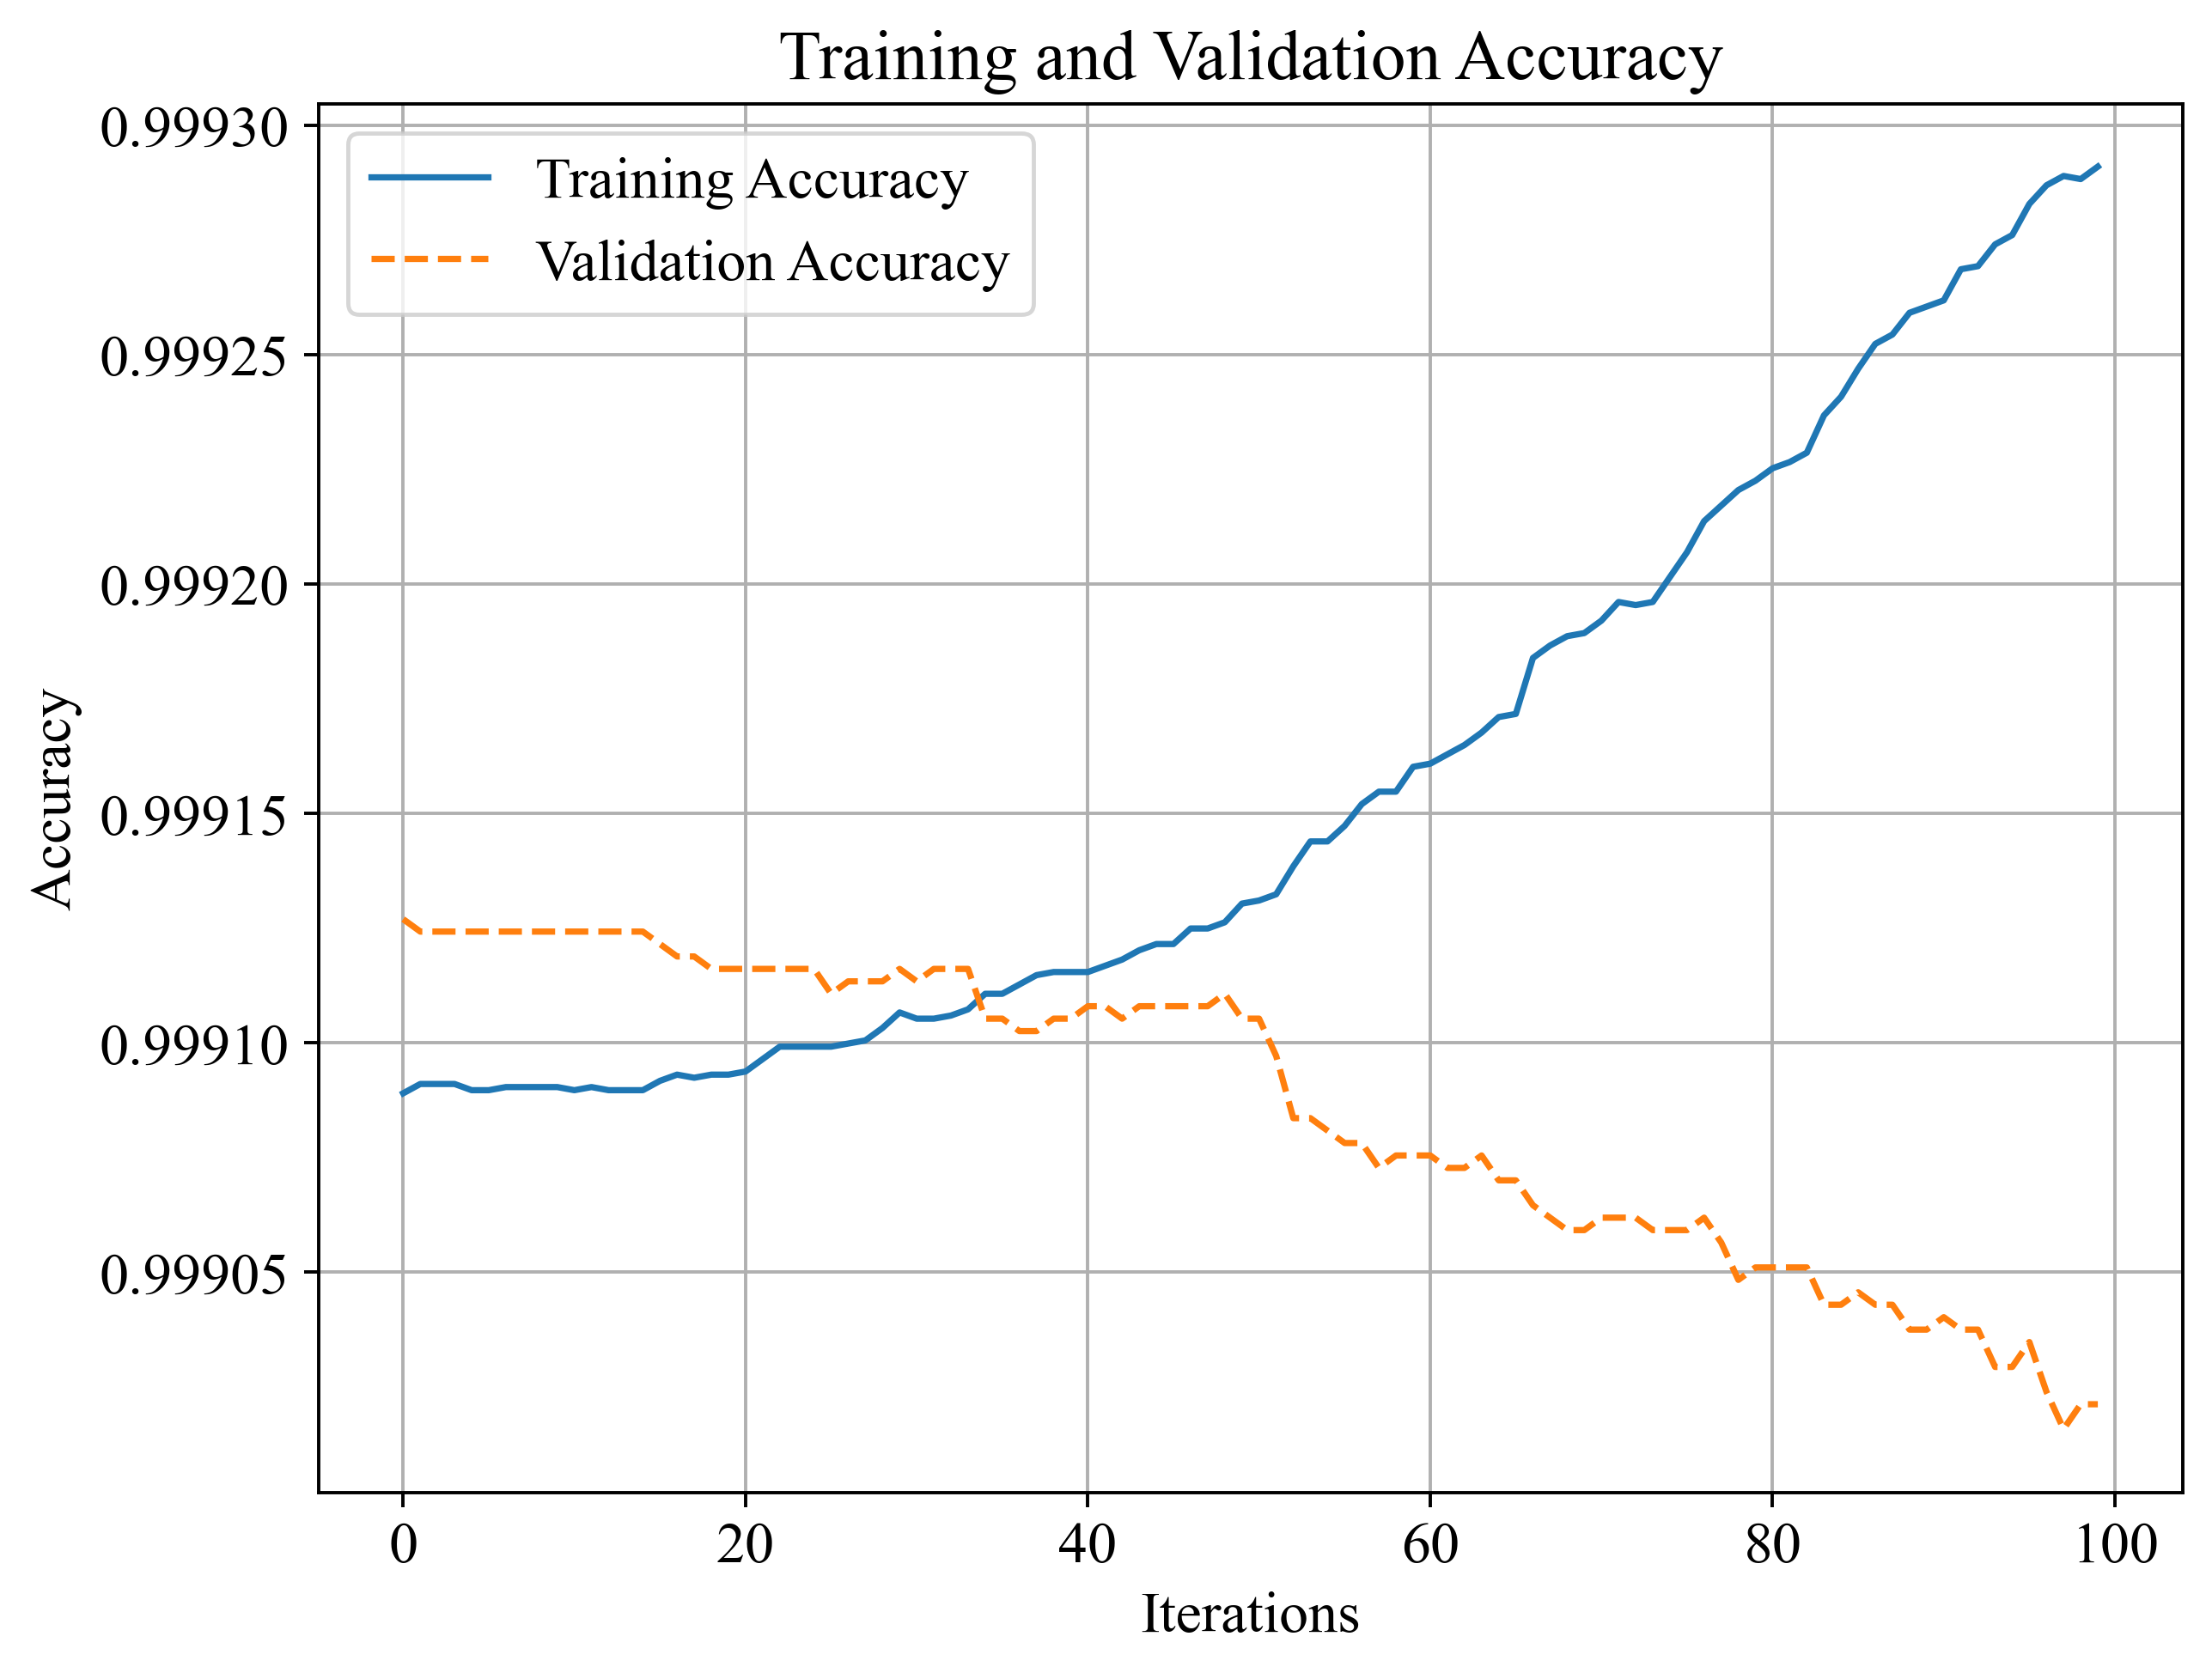
\includegraphics[width=0.8\textwidth]{media/ict/image40}
	\caption*{}
\end{figure}


{\bfseries Рис.5 - Динамика изменения потерь и результат точности для обучающей и валидационной выборки}

\begin{multicols}{2}
На рисунке 5 первый график изображает динамику изменения потерь (Log
Loss) на протяжении 100 итераций обучения модели. Синяя линия
представляет собой потери на обучающей выборке, а оранжевая -- на
валидационной. Можно заметить, что по мере увеличения количества
итераций потери на обеих выборках значительно уменьшаются и выходят на
плато, приближаясь к нулю. Это говорит о том, что модель успешно
обучается, минимизируя ошибки в прогнозировании как на тренировочных,
так и на валидационных данных, что указывает на хорошую способность
модели к обобщению. Стабилизация на низком уровне потерь свидетельствует
о высокой точности модели. Второй график на рисунке 5 демонстрирует
точность (Accuracy) для обучающей и валидационной выборок. Синяя линия
показывает, как растет точность модели на тренировочной выборке с
увеличением числа итераций, достигая практически 100\%. Однако для
валидационной выборки (оранжевая линия) наблюдается небольшое снижение
точности после 50 итераций, что может указывать на незначительное
переобучение модели. Тем не менее, обе линии остаются достаточно
высокими, что подтверждает эффективность модели. Процесс обучения модели
XGBoost проходит с хорошей конвергенцией: потери минимизируются, а
точность модели на тестовых данных остается на высоком уровне. Этот
результат указывает на то, что модель справляется с задачей
классификации эрозионных степеней, не только на тренировочных данных, но
и на новых данных, что делает её применимой для анализа и прогноза
деградации земельных участков в реальных условиях.

{\bfseries Выводы.} Данное исследование предложило эффективный подход к
выявлению и классификации эрозии почв с использованием данных
дистанционного зондирования и методов машинного обучения. Проблема
эрозии почв является одной из основных экологических угроз, снижая
плодородие земель и влияя на сельское хозяйство и устойчивость
экосистем. В ходе работы был разработан алгоритм, основанный на
комбинации спектральных индексов (NDVI, MSI, NDMI) и параметров альбедо,
что позволило разделить почву на четыре класса по степени эрозии:
«Норма», «Первая степень», «Вторая степень» и «Третья степень». Ключевым
аспектом методики является сочетание индексов растительности с оценкой
альбедо и влажности почвы, что позволяет избегать ошибочной
классификации участков, визуально похожих на эрозионные, но фактически
не подверженных эрозии.

Использование модели XGBoost для классификации эрозии почвы
продемонстрировало высокую эффективность, показывая точность как на
тренировочной, так и на тестовой выборках. Модель учитывает нелинейные
зависимости между входными признаками, что важно для анализа сложных
экологических процессов. Разработанная модель может быть полезна для
мониторинга больших территорий, подверженных эрозии, оперативно выявляя
участки, требующие восстановления. Методика имеет потенциал для
масштабных проектов по управлению земельными ресурсами и может быть
адаптирована для работы с другими регионами и типами данных. В будущем
важно рассмотреть возможность интеграции дополнительных спектральных
индексов и использования методов глубинного обучения для повышения
точности классификации и анализа сложных пространственно-временных
зависимостей в данных дистанционного зондирования.
\end{multicols}

\begin{center}
{\bfseries Литература}
\end{center}

\begin{references}
1. Жоголев А.В. Актуализация региональных почвенных карт на основе
спутниковых и геоинформационных технологий (на примере Московской
области): Автореф. дис. ... к. с.-х. н. - М., 2016. - 22 c.

2. Векшина В.Н. Построение цифровых моделей почвенного покрова западной
части Большеземельской тундры. Бюллетень Почвенного института имени
В.В. Докучаева.- 2019. Т.99.- С.21-46.
\href{https://doi.org/10.19047/0136-1694-2019-99-21-46}{DOI
10.19047/0136-1694-2019-99-21-46}.

3. Савин И.Ю., Прудникова Е.Ю. Об оптимальном сроке спутниковой съемки
для картографирования пахотных почв // Бюл. Почв. ин-та им. В.В.
Докучаева. -2014. -№ 74. -С.66-77.

4. Рожков В.А. Об информационном подходе в классификации почв//Бюллетень
Почвенного института имени В.В. Докучаева. -2012.-Т.(69).- С.4-24.
\href{https://doi.org/10.19047/0136-1694-2012-69-4-24}{DOI
/10.19047/0136-1694-2012-69-4-24}

5. Гребень А.С., Красовская И.Г. Анализ основных методик прогнозирования
урожайности с помощью данных космического мониторинга, применительно к
зерновым культурам степной зоны Украины // Радіоелектронні і
комп'ютерні системи. -2012. - № 2. - С.170-180.
\href{http://www.irbis-nbuv.gov.ua/cgi-bin/irbis_nbuv/cgiirbis_64.exe?I21DBN=LINK&P21DBN=UJRN&Z21ID=&S21REF=10&S21CNR=20&S21STN=1&S21FMT=ASP_meta&C21COM=S&2_S21P03=FILA=&2_S21STR=recs_2012_2_27}{http://nbuv.gov.ua}

6. Рожков В.А. Информатизация и теория классификации почв // Труды
Института государства и права РАН.- 2012.- № 6. -C.218-227

7. Hengl T., Mendes de Jesus J., Heuvelink G.B.M., Ruiperez Gonzalez M.,
Kilibarda M. SoilGrids250m: Global gridded soil information based on
machine learning // PLOS ONE. -2017. --Vol.12 (2):e0169748 DOI
10.1371/journal.pone.0169748

8. Чинилин А.В., Савин И.Ю. Крупномасштабное цифровое картографирование
содержания органического углерода почв с помощью методов машинного
обучения // Бюллетень Почвенного института им. В.В. Докучаева. -2018.
--Т.91. -- С.46-62. DOI 10.19047/0136-1694-2018-91-46-62

9. Masrur Ahmed, A.A., Deo, R.C., Raj, N., Ghahramani, A., Feng, Q., Yin,
Z., Yang, L. Deep learning forecasts of soil moisture: Convolutional
neural network and gated recurrent unit models coupled with
satellite-derived modis, observations and synoptic-scale climate index
data // Remote Sensing. -2021. --Vol.13 (554). -P.1-30. DOI
10.3390/rs13040554

10. Anton, C.A., Matei, O., Avram, A. Collaborative Data Mining in
Agriculture for Prediction of Soil Moisture and Temperature // Advances
in Intelligent Systems and Computing. -2019. -P.141-151. DOI
\end{references}

\begin{center}
{\bfseries References}
\end{center}

\begin{references}
1. Zhogolev A.V. Aktualizacija regional' nyh pochvennyh
kart na osnove sputnikovyh i geoinformacionnyh tehnologij (na primere
Moskovskoj oblasti): Avtoref. dis. ... k. s.-h. n. - M., 2016. - 22
s.{[}in Russian{]}

2. Vekshina V.N. Postroenie cifrovyh modelej pochvennogo pokrova zapadnoj
chasti Bol' shezemel' skoj tundry.
Bjulleten'{} Pochvennogo instituta imeni V.V.
Dokuchaeva.- 2019. T.99.- S.21-46. DOI \\10.19047/0136-1694-2019-99-21-46.
{[}in Russian{]}

3. Savin I.Ju., Prudnikova E.Ju. Ob optimal' nom sroke
sputnikovoj semki dlja kartografirovanija pahotnyh pochv // Bjul. Pochv.
in-ta im. V.V. Dokuchaeva. -2014. -№ 74. -S.66-77. {[}in Russian{]}

4. Rozhkov V.A. Ob informacionnom podhode v klassifikacii
pochv//Bjulleten'{} Pochvennogo instituta imeni V.V.
Dokuchaeva. -2012.-Т.69.- S.4-24. DOI /10.19047/0136-1694-2012-69-4-24.
{[}in Russian{]}

5. Greben'{} A.S., Krasovskaja I.G. Analiz osnovnyh
metodik prognozirovanija urozhajnosti s pomoshh' ju
dannyh kosmicheskogo monitoringa, primenitel' no k
zernovym kul' turam stepnoj zony Ukrainy //
Radіoelektronnі і komp'juternі sistemi. -2012. - №2. - S.170-180.
\href{http://www.irbis-nbuv.gov.ua/cgi-bin/irbis_nbuv/cgiirbis_64.exe?I21DBN=LINK&P21DBN=UJRN&Z21ID=&S21REF=10&S21CNR=20&S21STN=1&S21FMT=ASP_meta&C21COM=S&2_S21P03=FILA=&2_S21STR=recs_2012_2_27}{http://nbuv.gov.ua}. {[}in Russian{]}

6. Rozhkov V.A. Informatizacija i teorija klassifikacii pochv // Trudy
Instituta gosudarstva i prava RAN.- 2012.- № 6. -S.218-227. {[}in
Russian{]}

7. Hengl T., Mendes de Jesus J., Heuvelink G.B.M., Ruiperez Gonzalez M.,
Kilibarda M. SoilGrids250m: Global gridded soil information based on
machine learning // PLOS ONE. -2017. --Vol.12 (2):e0169748 DOI
10.1371/journal.pone.0169748

8. Chinilin A.V., Savin I.Ju. Krupnomasshtabnoe cifrovoe
kartografirovanie soderzhanija organicheskogo ugleroda pochv s
pomoshh' ju metodov mashinnogo obuchenija //
Bjulleten'{} Pochvennogo instituta im. V.V. Dokuchaeva.
-2018. --T.91. -- S.46-62. DOI 10.19047/0136-1694-2018-91-46-62. {[}in
Russian{]}

9. Masrur Ahmed, A.A., Deo, R.C., Raj, N., Ghahramani, A., Feng, Q., Yin,
Z., Yang, L. Deep learning forecasts of soil moisture: Convolutional
neural network and gated recurrent unit models coupled with
satellite-derived modis, observations and synoptic-scale climate index
data // Remote Sensing. -2021. --Vol.13 (554). -P.1-30. DOI
10.3390/rs13040554

10. Anton, C.A., Matei, O., Avram, A. Collaborative Data Mining in
Agriculture for Prediction of Soil Moisture and Temperature // Advances
in Intelligent Systems and Computing. -2019. -P.141-151. DOI
\end{references}

\begin{authorinfo}
\emph{{\bfseries Сведения об авторах}}

Болсынбек М. Қ. - докторант кафедры информационных систем Евразийского
национального университета имени Л. Н. Гумилева, Астана, Казахстан,
е-mail:

\href{https://orcid.org/0009-0001-0233-1984}{}

Абдикеримова Г.Б. - PhD, и.о. доцент кафедры информационных систем
Евразийского национального университета им.Л. Н.Гумилева, Астана,
Казахстан, е-mail:
\href{mailto:gulzira1981@mail.ru}{}{\bfseries ;
\href{https://orcid.org/0000-0002-4953-0737}{}}

Тасжурекова Ж.К. - к.т.н., и.о. доцента кафедры «Прикладная
информатика и программирование» Таразского регионального университета
им. М. Х. Дулати, Тараз, Казахстан, е-mail:

Адамов А.А. - д.т.н профессор, кафедра «Математическое и
компьютерное моделирование» член-корр. НИА РК, Евразийский национальный
университет им. Л.Н. Гумилева, Астана, Казахстан, е-mail:

\href{https://orcid.org/0000-0001-9515-1263}{}

Серикбаева С.К. - PhD, старший преподаватель кафедры информационных
систем Евразийского национального университета им. Л. Н. Гумилева,
Астана, Казахстан, е-mail:

Ануарбеков А.М. - Евразийский национальный университет имени
Л.Н.Гумилева, Преподаватель кафедры криптологии, Астана, Казахстан,
е-mail:
\href{mailto:almasanuarbekov01@gmail.com}{}.
\href{https://orcid.org/0009-0008-5013-3553}{}

\emph{{\bfseries Information about the authors}}

Bolsynbek M. - doctoral student of the Department of Information Systems
of the L. N. Gumilyov Eurasian National University, Astana, Kazakhstan,
е-mail: \href{mailto:mbolsynbek@bk.ru}{mbolsynbek@bk.ru};

Abdikerimova G.- PhD, acting associate professor of the Department of
Information Systems of L. N. Gumilyov Eurasian National University,
Astana, Kazakhstan, е-mail:
\href{mailto:gulzira1981@mail.ru}{gulzira1981@mail.ru};

Taszhurekova Zh. - acting associate professor of the Department «applied
informatics and programming» Taraz regional university named after M.
KH. Dulaty, Taraz, Kazakhstan. е-mail:

Adamov A. - Doctor of Technical Sciences, Professor, Department of
Mathematical and Computer Modeling, Corresponding Member, NIA RK, L.N.
Gumilyov Eurasian National University, Astana, Kazakhstan, е-mail:
adamov\_aa@enu.kz;

Serikbayeva S. - PhD, Senior Lecturer of the Department of Information
Systems, L.N. Gumilyov Eurasian National University, Astana, Kazakhstan.
E-mail:

Anuarbekov А. - L.N. Gumilyov Eurasian National University, Teacher,
Department of Cryptology, Astana, Kazakhstan, е-mail:
\href{mailto:almasanuarbekov01@gmail.com}{almasanuarbekov01@gmail.com}
\end{authorinfo}
